\section{Background}
\label{background}
In this section we give an overview of prior work 
and the context of this research.

\subsection{Rx in a nutshell}
To understand how we create the visualization a minimal understanding of RP and the chosen implementation is required. Many RP implementations share a notion of a \textit{Observable}, which is a collection which abstracts over \textit{time}, in contrast to \textit{space} like standard collections.

Figure \ref{sample1} shows a very basic example of a in situ data flow in Rx. First an \textit{Observable} is created, here using the static \code{from} method, then dependent Observables are created using the \code{map} and \code{filter} methods on the Observable instance. Finally we \code{subscribe} to start the data flow and send the data in the flow to the console (eg. JavaScript's stdout).

\begin{figure}
\inputminted[tabsize=2]{javascript}{listings/sample1.js}	
\caption{Creation and transform of Observables}
\label{sample1}
\end{figure}

It is important to note that the Observable is lazy, it is the blueprint of a data flow. Only when you \code{subscribe} to an Observable the data flow is created by recursively subscribing up the stream. \textit{Observer}s are subscribed to each Observable until the source Observable is reached.
This is illustrated in figure \ref{dualgraphs}.
The origin of this design is the duality between Observables and \textit{Iterables}~\cite{meijer2010subject}, where Observers are dual to \textit{Iterators}.

Creating the Observable we will call the \textit{assembly} phase, the phase where the subscribe happens the \textit{subscription} phase and data flows in the \textit{runtime} phase. The three phases can be interleaved for different streams, for example when dealing with higher order Observables,  meaning one could use Observables as values inside the data flow. The Observables used as values have yet to start the second phase while the outer stream is in the runtime phase.

\begin{figure}
\begin{verbatim}
TODO nice figure with Graph & 2 lines (1 up, 1 down)
^ from(1, 2, 3)   			
^ .map(x => x * 2)       v
^ .filter(x => x > 2)    v
  .subscribe()           v
\end{verbatim}
\caption{Observable \& Observer dependencies}
\label{dualgraphs}
\end{figure}


\subsubsection{Marble Diagram}
\label{marblediagram}
The term \textit{Marble Diagram} comes from the shape of the glyps in the images used to explain Rx in the official documentation. 
The diagrams contain one or more timelines containing the events that enter and leave Observables. 
Developers can see from the diagram how operators work by inspecting the difference between the timelines, 
where events might be skipped, added, transformed or delayed. 
Mapping time on the x-axis provides insight that is missing when inspecting only a single time slice, like with traditional debuggers.

\begin{figure}[ht]
\centering
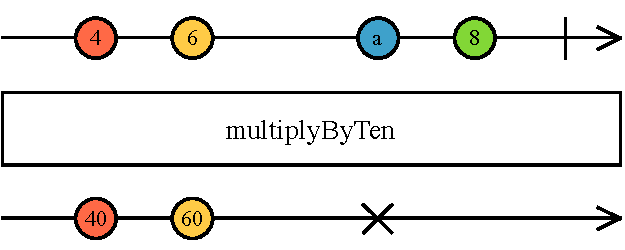
\includegraphics[width=\columnwidth]{images/marble-diagram.pdf}
\caption{Marble Diagram}
\label{marblediagram-image}
\end{figure}

\subsection{Debugging}
Debugging for general purpose languages revolves around 
attaching a debugger, 
stepping through the code, 
attaching code or data breakpoints, 
navigating along different calls in the call stack and 
examining variables and results of expressions~\cite{Spinellis2017}.
Existing research measuring how these different tasks are part of the developers work day found that 
while developers spend much time on comprehending code they do not spend much time inside the debugger~\cite{minelli2015know}.
Beller et al.~\cite{beller2017behavior} found that only 23\% of their subjects actively use the debugger,
with the most common action being adding breakpoints, followed by stepping through code.
The automated tooling of these studies did not measure different kinds of debugging other than using the IDE provided tools, 
however Beller's survey indicates that 71\% also uses printf statements for debugging.  
No indication was given of the language and libraries used by the subjects in the study, 
but the observation that printf debugging is common matches our experience with debugging reactive programs.

% What comprises debugging?
% \item Maybe Zeller / Spinellis?

% \item Petrillo, ``Towards Understanding..." e.g. Swarm debugging
% \item Minelli (know what you did last summer)
% \item Moritz (watchdog 2.0)

\subsection{Debugging for Program Comprehension}
Both debugging and comprehension are processes in the work of programmers.
Initially comprehension was seen as a distinct step programmers had to make
prior to being able to debug programs~\cite{katz1987debugging}, 
but this distinction is criticized by Gilmore saying we must view 
``debugging as a design activity''~\cite{gilmore1991models}, 
part of creating and comprehending programs. 
Maalej et al.~\cite{Maalej2014} interviewed professional developers 
and found that developers require runtime information to understand a program,
and that debugging is frequently used to gather this runtime information.
This supports our view that `debugging' is not only used for fault localization,
but also for comprehension.

% \item Katz, distinct step
% \item Gilmore, comprehension + debugging == linked
% \item Maalej: professionals, avoid deep comprehension, sharing knowlegde

